\documentclass[11pt]{article}

\usepackage{mathnotes}
\pgfplotsset{compat=1.18}

% Title Information
\title{\Huge  \color{HTML}{5A0000} Notas de Cálculo Avanzado}
\author{Ramiro Dibur}
\date{}

% Document

\begin{document}

\pagenumbering{gobble}
\vspace*{\fill}
\begin{center}
    \vspace*{\stretch{1}}
    {\Huge  Notas de Cálculo Avanzado} \\[1em]
    {\large Ramiro Dibur}
    \vspace*{\stretch{2}}
\end{center}
\vspace*{\fill}
\newpage
\pagenumbering{arabic}
\newpage
\tableofcontents
\newpage

% -------------

% \section{Teoría de Conjuntos}

Lo básico de teoría de conjuntos (definición de conjunto, partes de un conjunto, intersección, unión, \dots) es algo ya visto en Álgebra I y utilizado frecuentemente en Álgebra Lineal. Por lo tanto, no vamos a ver nada al respecto.  

\subsection{Relaciones}

Si bien relaciones lo vimos en Álgebra I, amerita un breve repaso de las definiciones y propiedades básicas.

\begin{definition}
    Una \emph{relación} binaria $\mathcal{R}$ entre $A$ y $B$ es un subconjunto de $A \times B$. Decimos que $a \mathcal{R} b$ si $(a, b) \in A \times B$.
\end{definition}

En particular, vamos a tratar con las relaciones en $A \times A$, a las cuales les decimos simplemente relaciones en $A$.

Un ejemplo clásico de relación es la relación de igualdad en un conjunto $A$, definida como el conjunto $\{(a, a) \mid a \in A\}$. En otras palabras, cada elemento de $A$ está relacionado únicamente consigo mismo, y no con ningún otro elemento.

Nos interesa categorizar algunas relaciones en particular. 

\begin{definition}
    Una relación $\mathcal{R}$ en $A$ es de \emph{equivalencia} si satisface las siguientes propiedades:
    \begin{itemize}
        \item \textbf{Reflexiva}: Para todo $a \in A$, se cumple que $a \mathcal{R} a$.
        \item \textbf{Simétrica}: Para todo $a, b \in A$, si $a \mathcal{R} b$, entonces $b \mathcal{R} a$.
        \item \textbf{Transitiva}: Para todo $a, b, c \in A$, si $a \mathcal{R} b$ y $b \mathcal{R} c$, entonces $a \mathcal{R} c$.
    \end{itemize}
\end{definition}

La relación de igualdad cumple la definición de relación de equivalencia de forma trivial. Otra relación de equivalencia que no es trivial es la congruencia módulo $n$.

\begin{example}
    Decimos que $m, n \in \mathbb{Z}$ son congruentes módulo $N \in \mathbb{N}$ si ambos tienen el mismo resto al dividirlos por $N$ y la denotamos como
    $$
        m \equiv n \pmod{N}.
    $$
\end{example}

La demostración de que es una relación de equivalencia le queda al lector.

Por otro lado, tenemos las relaciones de orden.

\begin{definition}
    Una relación $\mathcal{R}$ en $A$ es de \emph{orden} si satisface las siguientes propiedades:
    \begin{itemize}
        \item \textbf{Reflexiva}: Para todo $a \in A$, se cumple que $a \mathcal{R} a$.
        \item \textbf{Anti-simétrica}: Para todo $a, b \in A$, si $a \mathcal{R} b$ y $b \mathcal{R} a$, entonces $a = b$.
        \item \textbf{Transitiva}: Para todo $a, b, c \in A$, si $a \mathcal{R} b$ y $b \mathcal{R} c$, entonces $a \mathcal{R} c$.
    \end{itemize}
\end{definition}

De ahora en adelante, utilizaremos $\preceq$ para denotar a una relación de orden arbitraria.

Estas relaciones son las que nos interesan en Cálculo Avanzado. Un ejemplo trivial de relación de orden son los números reales $\mathbb{R}$ junto con la relación $ \leq $. Otra relación quizás no tan aparente es la de los naturales $N$ junto con la divisibilidad.

\begin{example}
    Sean $m, n \in \mathbb{N}$. Decimos que $m$ divide a $n$ si el resto de $n$ al dividirlo por $m$ es $0$ y lo denotamos como
    $$
        m \mid n.
    $$
\end{example}

La demostración queda para el lector.

\subsection{Conjuntos ordenados}

Veamos la definición de un conjunto ordenado.

\begin{definition}
    Decimos que un conjunto $A$ junto con una relación de orden $\preceq$ es un \emph{conjunto ordenado} (o \emph{poset}) y lo denotamos como $(A, \preceq)$.
\end{definition}

La palabra \textit{poset} viene del inglés ``partially ordered set''.

\begin{definition}
    Sea $(A, \preceq)$ un conjunto ordenado. Si para todo $a, b \in A$ se cumple $a \preceq b$ o $b \preceq a$, decimos que $A$ es un conjunto \emph{totalmente ordenado} (o \emph{cadena}). Sino, decimos que es un conjunto \emph{parcialmente ordenado}.
\end{definition}

Algunos ejemplos de orden parcial son:
\begin{itemize}
    \item El conjunto de partes de un conjunto junto con el orden de inclusión $(\mathcal{P}(X), \subseteq)$.
    \item El conjunto de los números naturales junto con la relación de divisibilidad $(\mathbb{N}, \mid)$.
\end{itemize}
Y otros ejemplos de conjuntos totalmente ordenados:
\begin{itemize}
    \item El conjunto de los números reales junto con la relación de orden usual $(\mathbb{R}, \leq)$.
    \item El conjunto de las palabras en un diccionario ordenadas alfabéticamente.
\end{itemize}


\subsection{Reticulados}

\begin{definition}
    Decimos que un conjunto ordenado $(\mathcal{O}, \preceq)$ es un \emph{reticulado} si para todo $a, b \in \mathcal{O}$ existen:
    \begin{itemize}
        \item Un \emph{supremo} denotado como $a \vee b$, que es el menor elemento de $\mathcal{O}$ que es mayor o igual que $a$ y $b$.
        \item Un \emph{ínfimo} denotado como $a \wedge b$, que es el mayor elemento de $\mathcal{O}$ que es menor o igual que $a$ y $b$.
    \end{itemize}
\end{definition}

Algunos ejemplos de reticulados son:
\begin{itemize}
    \item El conjunto de partes de un conjunto $(\mathcal{P}(X), \subseteq)$, donde el supremo es la unión de conjuntos $A \vee B = A \cup B$ y el ínfimo es la intersección $A \wedge B = A \cap B$.
    \item El conjunto de números enteros $(\mathbb{Z}, \leq)$, donde el supremo es el máximo de dos números $a \vee b = \max(a, b)$ y el ínfimo es el mínimo $a \wedge b = \min(a, b)$.
    \item El conjunto de divisores de un número natural $n$ con la relación de divisibilidad $(D(n), \mid)$, donde el supremo es el mínimo común múltiplo $a \vee b = \operatorname{mcm}(a, b)$ y el ínfimo es el máximo común divisor $a \wedge b = \operatorname{mcd}(a, b)$.
\end{itemize}

\begin{remark}
    En un reticulado no necesariamente existe el supremo de un conjunto infinito. Por ejemplo, en el reticulado $(\mathbb{N}, \leq)$, el conjunto de los números enteros positivos no tiene un supremo, ya que no existe un número entero que sea mayor o igual a todos los números positivos.
\end{remark}

Lo cual nos lleva a la siguiente definición.

\begin{definition}
    Un reticulado $(\mathcal{O}, \preceq)$ es \emph{completo} si para todo subconjunto no vacío de $\mathcal{O}$ existe su supremo e ínfimo.
\end{definition}

Algunos ejemplos de reticulados completos son:
\begin{itemize}
    \item El conjunto de partes de un conjunto $(\mathcal{P}(X), \subseteq)$, ya que para cualquier colección de subconjuntos, siempre existen la unión (supremo) y la intersección (ínfimo).
    \item El conjunto de números reales extendido con $+\infty$ y $-\infty$ $(\mathbb{R} \cup \{-\infty, +\infty\}, \leq)$, donde cualquier subconjunto tiene un supremo e ínfimo.
\end{itemize}

A continuación veremos algunas propiedades básicas de reticulados las cuales no voy a demostrar.

\begin{proposition}
    Sea $(\mathcal{O}, \preceq)$ un reticulado. Entonces, las siguientes propiedades son verdaderas:
    \begin{enumerate}
        \item \textbf{Idempotencia:} $a \vee a = a$ y $a \wedge a = a$.
        \item \textbf{Conmutatividad:} $a \vee b = b \vee a$ y $a \wedge b = b \wedge a$.
        \item \textbf{Asociatividad:} $(a \vee b) \vee c = a \vee (b \vee c)$ y $(a \wedge b) \wedge c = a \wedge (b \wedge c)$.
        \item \textbf{Absorción:} $a \vee (a \wedge b) = a$ y $a \wedge (a \vee b) = a$.
    \end{enumerate}
\end{proposition}

\subsection{Reticulados finitos}

Tal como dice el nombre:

\begin{definition}
    Un reticulado $(\mathcal{O}, \preceq)$ es \emph{finito} si $\mathcal{O}$ es finito.
\end{definition}

Los reticulados finitos los podemos representar con un \textit{diagrama de Hasse}. Un diagrama de Hasse es un grafo donde cada vértice representa un elemento y las aristas, una relación entre dos elementos.

Por ejemplo, consideremos el reticulado $(D(18), \mid)$. Lo podemos representar con un diagrama de Hasse de la siguiente manera:

\begin{figure}
    \centering
    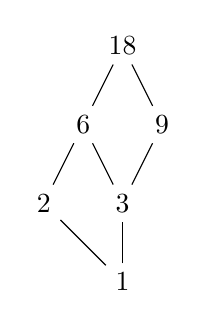
\begin{tikzpicture}[scale=0.5]
        \node (1) at (0,0) {$1$};
        \node (2) at (-2,2) {$2$};
        \node (3) at (0,2) {$3$};
        \node (6) at (-1,4) {$6$};
        \node (9) at (1,4) {$9$};
        \node (18) at (0,6) {$18$};
    
        \draw (1) -- (2);
        \draw (1) -- (3);
        \draw (2) -- (6);
        \draw (3) -- (6);
        \draw (3) -- (9);
        \draw (6) -- (18);
        \draw (9) -- (18);
    \end{tikzpicture}
    \caption{Diagrama de Hasse del reticulado $(D(18), \mid)$.}
\end{figure}

Notemos que únicamente están conectados los vértices $x$ e $y$ para los cuales no existe $z$ tal que $x \mid z \mid y$. Y las aristas siempre van hacia arriba.

A su vez, el diagrama de Hasse nos facilita ver una propiedad interesante: todo reticulado finito es completo.

\begin{proposition}
    Sea $(\mathcal{O}, \preceq)$ un reticulado \textit{finito} y no vacío. Entonces es completo.
\end{proposition}

\begin{proof}
    Sea $X = \set{ x_{1}, x_{2}, \dots, x_{n} }$ un subconjunto de $\mathcal{O}$. Procedemos por inducción en el cardinal del subconjunto. 

    Para $\lvert X \rvert = 1$, el supremo de $X$ es su único elemento.

    Supongamos que para todo subconjunto con cardinal menor a $n$ existe supremo. Defino $Y = \set{ x_{1}, x_{2}, \dots, x_{n-1} \vee x_{n} }$. Por definición de supremo,
    $$
        x_{1}, x_{2}, \dots, x_{n-2} \preceq \sup Y,
    $$
    y también
    $$
    x_{n-1}, x_{n} \preceq x_{n-1} \vee x_{n} \preceq \sup Y.
    $$
    Por lo tanto
    $$
        x_{1}, x_{2}, \dots, x_{n} \preceq \sup Y,
    $$
    Entonces, $\sup Y$ es cota superior de $X$. Sea $c$ una cota superior de $X$. En particular, $x_{n-1} \vee x_{n} \preceq c$ ya que $x_{n-1}, x_{n} \preceq c$. Por lo tanto, $c$ también es una cota de $Y$, entonces $\sup Y \preceq c$. Demostrando que $\sup X = \sup Y$. La demostración para el ínfimo es análoga.
\end{proof}

\subsection{Morfismos de orden}

Consideremos una función entre conjuntos ordenados
$$
    f: (A, \preceq_{A}) \to (B, \preceq_{B}).
$$
Por comodidad, directamente vamos a escribir
$$
    f: A \to B.
$$
Y además utilizaremos el mismo símbolo $\preceq$ para $\preceq_{A}$ y $\preceq_{B}$. Por lo general no genera confusión, pero en el caso que sí, se aclarará qué orden se utiliza.

\begin{definition}
    Sean $A$ y $B$ conjuntos ordenados. Decimos que una función $f: A \to B$ es un \emph{morfismo de orden} (o \emph{creciente}) si se cumple que
    \begin{center}
        si $a \preceq a'$ en $A$, entonces $f(a) \preceq f(a')$ en $B$.
    \end{center}
    Y \emph{decreciente} si se cumple que 
    \begin{center}
        si $a \preceq a'$ en $A$, entonces $f(a) \succeq f(a')$ en $B$.
    \end{center}
\end{definition}

Por ejemplo, la función $\operatorname{Id}: (\mathbb{N}, \mid ) \to (\mathbb{N}, \leq)$ es un morfismo de orden, ya que si $m \mid n$ entonces $m \leq n$.

\begin{remark}
    No necesariamente es verdadera la vuelta. Esto se ve fácil con el ejemplo de arriba si tomamos $m = 2$ y $n = 3$, $2 \leq 3$ pero $2 \nmid 3$.
\end{remark}

Para eso definimos un isomorfismo de orden.

\begin{definition}
    Sean $A$ y $B$ conjuntos ordenados. Decimos que una función \textit{biyectiva} $f: A \to  B$ es un \emph{isomorfismo de orden} si se cumple que
    \begin{center}
        $a \preceq a'$ si y sólo si $f(a) \preceq f(a')$.
    \end{center}
\end{definition}

\begin{remark}
    Esto es lo mismo que decir que $f$ y $f^{-1}$ son ambas morfismos de orden.
\end{remark}

Veamos algunos ejemplos de isomorfismos de orden:

\begin{itemize}
    \item La función $f: (\mathbb{R}, \leq) \to (\mathbb{R}_{>0}, \leq)$ tal que $f(x) = e^x$.
    \item La función $f: (\mathbb{Z}, \leq) \to (2\mathbb{Z}, \leq)$ tal que $f(x) = 2x$.
    \item La función $f: (\mathcal{P}(X), \subseteq) \to (\mathcal{P}(X), \supseteq)$ tal que $f(A) = X \setminus A$.
\end{itemize}

A continuación demostramos el teorema del punto fijo para reticulados completos.

\begin{theorem}
    Sea $(\mathcal{O}, \preceq)$ un reticulado \textit{completo} y sea $f: \mathcal{O} \to  \mathcal{O}$ un \textit{morfismo de orden}. Entonces, existe $x \in \mathcal{O}$ tal que $f(x)= x$.
\end{theorem} 

\begin{proof}
    Sea $A = \set{ x \in \mathcal{O} \mid x \preceq f(x) }$. Como $\mathcal{O}$ es un reticulado completo, considero $s = \sup A$. Recordemos que, para todo $a \in A$, $a \preceq s$. Y como $f$ es creciente, para todo $a \in A$, 
    $$
        f(a) \preceq f(s).
    $$
    Por definición de $A$, $a \preceq f(a)$ y a su vez $f(a) \preceq f(s)$, entonces, para todo $a \in A$,
    $$
        a \preceq f(s).
    $$
    O sea, $f(s)$ es cota superior de $A$. Por definición del supremo, $s \preceq f(s)$ y entonces $s \in A$. A la desigualdad $s \preceq f(s)$ le aplicamos $f$ y obtenemos
    $$
        f(s) \preceq f(f(s)).
    $$
    Por lo tanto, $f(s) \in A$; entonces tenemos $f(s) \preceq s$ y $s \preceq f(s)$, lo cual implica que $f(s) = s$.
\end{proof}

\subsection{Cardinalidad}

\begin{definition}
    Decimos que un conjunto $A$ es \emph{finito} si es vacío o existe una biyección $f: \llbracket n \rrbracket \to  A$. Definimos $\# A = n$ y $\# \emptyset = 0$. Además, $A$ es \emph{infinito} si no es finito.
\end{definition}

\begin{remark}
    La definición de $\# A$ tiene sentido dado que $f: \llbracket m \rrbracket \to \llbracket n \rrbracket$ es biyectiva si y sólo si $m = n$.
\end{remark}

\begin{definition}
    Decimos que $A$ es \emph{numerable} si existe una biyección $f: \mathbb{N} \to  A$. Además, si $A$ es numerable o finito decimos que es \emph{contable}.
\end{definition}

Algunos ejemplos de conjuntos numerables son:

\begin{itemize}
    \item El conjunto $2 \mathbb{N}$.
    \item El conjunto de números primos.
    \item Los conjuntos $\mathbb{Z}$ y $\mathbb{Q}$.
\end{itemize}

\begin{definition}
    Si existe $f: A \to  B$ biyectiva, entonces se dice que $A$ y $B$ son \emph{coordinables} y lo denotamos como $A \sim B$.
\end{definition}

\begin{remark}
    Todo conjunto numerable es coordinable con $\mathbb{N}$ y \textit{viceversa}.
\end{remark}

\begin{lemma}
    Todo subconjunto $A \subseteq \mathbb{N}$ es contable.
\end{lemma}

\begin{proof}
    Si $A$ es finito, entonces ya estamos. Supongamos que $A$ es infinito. Defino la función $f: \mathbb{N} \to A$ tal que $f(1) = \min A$ y 
    $$
        f(n+1) = \min (A - \set{ f(1), f(2), \dots, f(n) }).
    $$
    Como $A$ es infinito, $f$ está bien definida. Además, $f$ es claramente una biyección. Por lo tanto, $A$ es contable.
\end{proof}

\begin{proposition}
    Sea $X$ un conjunto \textit{numerable}. Si existe $f: X \twoheadrightarrow Y$ sobreyectiva, entonces $Y$ es contable. 
\end{proposition}

\begin{proof}
    Si $X \neq \mathbb{N}$ simplemente consideramos una biyección de $\mathbb{N}$ a $X$. Entonces, podemos suponer que $X = \mathbb{N}$. 
        
    Sea $f: X \twoheadrightarrow Y$ sobreyectiva. Definimos la función
    $$
        g: Y \to \mathbb{N} \text{ tal que } y \mapsto \min f^{-1}(y).
    $$
    La función $g$ está bien definida porque $f$ es sobreyectiva, lo que garantiza que $f^{-1}(y) \neq \emptyset$ para todo $y \in Y$. Como $g$ es inyectiva, la restricción $g|_{\operatorname{Im}g}$ es biyectiva. Dado que encontramos una biyección entre $Y$ y un subconjunto de $\mathbb{N}$, demostramos que $Y$ es contable.
\end{proof}

\begin{example}
    Los conjuntos $\mathbb{N} \times \mathbb{N}$ y $\mathbb{N}$ son coordinables.
\end{example}

\begin{proof}[Solución]
    Definimos la función 
    $$
        \Phi : \mathbb{N} \times \mathbb{N} \to \mathbb{N} \text{ tal que }\Phi (m, n) = 2^{m} 3^{n}.
    $$
    Dada la factorización única de los naturales, $\mathbb{N} \times \mathbb{N}$ es coordinable con un subconjunto de $\mathbb{N}$. Por lo tanto, es contable. Claramente, como $\operatorname{Im} \Phi$ no es finito, $\mathbb{N} \times \mathbb{N}$ es numerable.
\end{proof}

\begin{example}
    Los conjuntos $\mathbb{N}$ y $\mathbb{R}$ no son coordinables.
\end{example}

\begin{proof}[Solución]
    Supongamos que $\mathbb{N} \sim \mathbb{R}$. Para facilitarnos la vida, podemos considerar la biyección $g: \mathbb{R} \to (0, 1)$ dada por $g(x) = \frac{\tan^{-1} (x)}{\pi} + \frac{1}{2}$.

    \begin{figure}[H]
        \centering
        \begin{tikzpicture}
            \begin{axis}[
            axis lines = middle,
            xlabel = {$x$},
            ylabel = {$g(x)$},
            ymin = 0, ymax = 1,
            xmin = -10, xmax = 10,
            samples = 100,
            domain = -10:10,
            width = 10cm,
            height = 5cm,
            ytick = \empty,
            xtick = \empty
            ]
            \addplot[emphcolor, thick] {rad(atan(x))/pi + 0.5};
            \addplot[dashed, gray] {0};
            \addplot[dashed, gray] {1};
            \end{axis}
        \end{tikzpicture}
        \caption{Gráfico de la función $g(x) = \frac{\tan^{-1}(x)}{\pi} + \frac{1}{2}$.}
    \end{figure}

    Por lo tanto, basta con demostrar que no existe una biyección entre $\mathbb{N}$ y $(0, 1)$. Sea $f: \mathbb{N} \to (0, 1)$ una biyección tal que
    \begin{align*}
        f(1) &= 0.a_{11}a_{12}a_{13}\dots \\
        f(2) &= 0.a_{21}a_{22}a_{23}\dots \\
        f(3) &= 0.a_{31}a_{32}a_{33}\dots \\
             &\dots
    \end{align*}
    Consideramos el número definido por agarrar los dígitos de la diagonal y sumarle $1$ si es menor que $9$ o restarle $1$ si es $9$. Nos queda el número
    $$
        0.a'_{11}a'_{22}a'_{33}\dots
    $$
    Este número es distinto $f(n)$ en el $n$-ésimo dígito decimal. Lo cual es absurdo, ya que si $f$ es biyectiva debería existir un natural $m$ tal que $f(m) = 0.a'_{11}a'_{22}a'_{33}\dots$. Por lo tanto, demostramos que $\mathbb{N}$ no es coordinable con $\mathbb{R}$.
\end{proof}

Probaremos el teorema de Schröder–Bernstein que va a facilitarnos la vida significativamente. Hasta ahora, para verificar si dos conjuntos eran coordinables era necesario encontrar una biyección entre los conjuntos. Esto nos ahorra tener que encontrar la biyección y sólo nos requiere encontrar dos funciones inyectivas.

\begin{theorem}
    Sean $f: X \hookrightarrow Y$ y $g: Y \hookrightarrow X$ funciones \textit{inyectivas}. Entonces, existe una biyección $h: X \to  Y$.
\end{theorem}

\begin{proof}
    La idea detrás de esta demostración es particionar a los conjuntos $X$ e $Y$ en $A$, $B$ y $A'$, $B'$, respectivamente, de forma tal que 
        $$
            A \cap B = A' \cap B' = \emptyset,
        $$
        y
        $$
            A \cup B = X \quad \text{y} \quad A' \cup B' = Y,
        $$
        y además
        $$
            f(A) = A' \quad \text{y} \quad f(B) = B'.
        $$
    \begin{figure}[H]
        \centering
        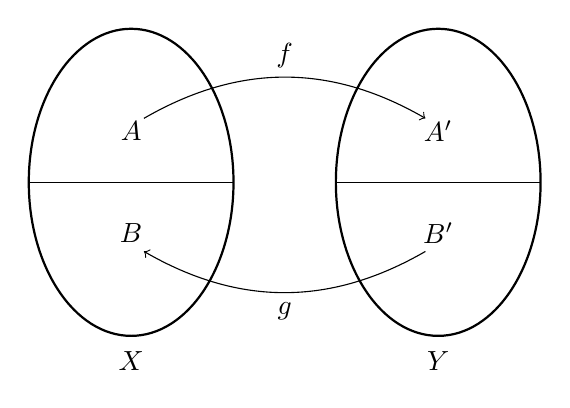
\begin{tikzpicture}[scale=0.65]
            % Sets X and Y
            \draw[thick] (0,0) ellipse (2 and 3);
            \draw[thick] (6,0) ellipse (2 and 3);
            
            % Labels for X and Y
            \node at (0,-3.5) {$X$};
            \node at (6,-3.5) {$Y$};
            
            % Subsets A and B in X
            \node at (0,1) {$A$};
            \node at (0,-1) {$B$};
            
            % Subsets A' and B' in Y
            \node at (6,1) {$A'$};
            \node at (6,-1) {$B'$};
            
            % Diagonal line between X and Y
            \draw (-2, 0) -- (2, 0);
            \draw (4, 0) -- (8, 0);
            
            \draw[-to, bend left] (0.25,1.25) to node[midway, above] {$f$} (5.75,1.25);
            \draw[-to, bend left] (5.75,-1.35) to node[midway, below] {$g$} (0.25,-1.35);
        \end{tikzpicture}
        \caption{Partición de los conjuntos $X$ e $Y$ en $A$, $B$ y $A'$, $B'$.}
    \end{figure}

    Esto se reduce a encontrar $A \subseteq X$ tal que
    $$
        X - g(Y - f(A)) = A.
    $$
    Definimos $\Phi : \mathcal{P}(X) \to  \mathcal{P}(X)$ tal que $\Phi(A) = X - g(Y - f(A))$. Lo cual nos da la siguiente ecuación,
    $$
        \Phi (A) = A.
    $$
    Veamos que $\Phi$ es un morfismo de orden con en $(\mathcal{P}(X), \subseteq )$. Sean $X_{0}$ y $X_{1}$ subconjuntos de $X$. Supongamos que $X_{0} \subseteq X_{1}$. Entonces,
    \begin{align*}
        X_{0} &\subseteq X_{1} \\
        f(X_{0}) &\subseteq f(X_{1}) \\
        Y - f(X_{0}) &\supseteq Y - f(X_{1}) \\
        g(Y - f(X_{0})) &\supseteq g(Y - f(X_{1})) \\
        X - g(Y - f(X_{0})) &\subseteq X - g(Y - f(X_{1})) \\
        \Phi(X_{0}) & \subseteq \Phi(X_{1})
    \end{align*}
    probando que $\Phi$ es un morfismo de orden. Y como ya sabemos, $(\mathcal{P}(X), \subseteq)$ es un reticulado completo. Por lo tanto, podemos utilizar el teorema del punto fijo, dándonos un $A \subseteq X$ tal que $\Phi (A) = A$.
\end{proof}

\begin{example}
    El conjunto $\set{ 0, 1 }^{\mathbb{N}}$ es coordinable con $\mathbb{R}$.
\end{example}

\begin{proof}[Solución]
    Probamos que $\set{ 0, 1 }^{\mathbb{N}} \sim [0, 1] \sim \mathbb{R}$. 
    
    Para $\set{ 0, 1 }^{\mathbb{N}} \hookrightarrow [0, 1]$ tomamos la escritura en base $10$. Y para $[0, 1] \hookrightarrow \set{ 0, 1 }^{\mathbb{N}}$ tomamos la escritura en base $2$.
\end{proof}

\begin{theorem}
    Todo conjunto $X$ no es coordinable con $\mathcal{P}(X)$.
\end{theorem}

\begin{proof}
    Supongamos que $X \sim \mathcal{P}(X)$. Entonces, existe una función biyectiva $f: \mathcal{P}(X) \to X$. Sea 
    $$
        Y = \set{ x \in X \mid x \not \in g(X)}.
    $$
    Consideramos $y = f(Y) \in X$. Como $f$ es biyectiva, $f^{-1}(y) = Y$. Con esto llegamos a un absurdo.
    \begin{center}
        Si $y \in Y$, entonces $y \not \in f^{-1}(y) = Y$.

        Si $y \not \in Y$, entonces $y \in f^{-1}(y) = Y$.
    \end{center}
    En ambos casos, llegamos a un absurdo. Entonces, nuestra suposición inicial de que $X \sim \mathcal{P}(X)$ es falsa.
\end{proof}

\subsection{Axioma de elección y lema de Zorn}

En estas notas (y en la cursada) se acepta el axioma de elección y el principio de buena ordenación. El axioma de elección postula lo siguiente.
\begin{custombox}[Axioma de elección]
    Sea $\mathcal{F}$ una familia de conjuntos no vacíos y disjuntos dos a dos. Entonces, existe una función $f: \mathcal{F} \to \bigcup \mathcal{F}$ tal que $f(A) \in A$ para todo $A \in \mathcal{F}$.
\end{custombox}

Otras formulaciones equivalentes son:
\begin{enumerate}[label=(\roman*)]
    \item Sea $X$ un conjunto. Existe una función
    $$f: \mathcal{P}(X) - \set{ \emptyset } \to X$$ 
    tal que $f(A) \in A$ para todo $A \in \mathcal{P}(X)$.   
    \item El producto cartesiano de conjuntos no vacíos es no\\ vacío.
\end{enumerate}

El axioma de elección también es equivalente al principio de buena ordenación.

\begin{custombox}[Principio de buena ordenación]
    Todo conjunto puede ser dotado de un orden tal que todo subconjunto no vacío tiene un elemento mínimo. A este tipo de orden se le llama \textit{orden bueno}.
\end{custombox}

Aceptando el axioma de elección (y en consecuencia el principio de buen ordenamiento) se puede demostrar el lema de Zorn.

\begin{custombox}[Lema de Zorn]
    Son equivalentes:
    \begin{enumerate}[label=(\roman*)]
        \item Sea $(A, \preceq)$ un conjunto parcialmente ordenado tal que toda cadena de $A$ tiene cota superior. Entonces, $A$ tiene un elemento maximal.
        \item Sea $(A, \preceq)$ un conjunto parcialmente ordenado tal que toda cadena de $A$ tiene supremo. Entonces, $A$ tiene un elemento maximal.
        \item Todo conjunto parcialmente ordenado tiene una cadena maximal.
    \end{enumerate}
\end{custombox}

\subsection{Aritmética de cardinales}

Cuando trabajamos con cardinales de conjuntos, para probar que dos conjuntos tienen el mismo cardinal es necesario establecer una biyección o inyecciones hacia ambos lados. Sin embargo, encontrar la función en particular puede ser molesto a veces. Para esto sirve la aritmética de cardinales. Nos ahorra el trabajo de encontrar una función en particular y nos permite trabajar con cardinales generales.

\begin{definition}
    Decimos que dos conjuntos $A$ y $B$ tienen el mismo \emph{cardinal} si existe una función biyectiva $f: A \to  B$ y lo denotamos como $\lvert A \rvert = \lvert B \rvert$.
\end{definition}

Por ejemplo, si $A$ es un conjunto numerable, entonces
$$
    \lvert A \rvert = \lvert \mathbb{N} \rvert.
$$
En general, como hay algunos cardinales que son más ocurrentes, los denotamos de una forma especial.

\begin{definition}
    Denotamos
    \begin{itemize}
        \item El cardinal de $\mathbb{N}$ como $\aleph_0$.
        \item El cardinal de $\mathbb{R}$ como $\mathfrak{c}$.
    \end{itemize}
\end{definition}

\begin{remark}
    Si $A$ es numerable, entonces su cardinal es $\aleph_0$.
\end{remark}

\begin{definition}
    Sean $A$ y $B$ conjuntos. Si existe una función inyectiva $f: A \hookrightarrow B$, entonces $\lvert A \rvert \leq \lvert B \rvert$.
\end{definition}

Si bien tratamos con funciones inyectivas, podríamos haber utilizado funciones sobreyectivas para las definiciones; ya que, si existe $f: A \hookrightarrow B$ inyectiva y $A \neq \emptyset $, entonces existe $g: B \twoheadrightarrow A$ sobreyectiva.

A continuación veremos una suerte de tricotomía pero para los cardinales. Para la demostración de este teorema, es necesario el lema de Zorn. 

\begin{theorem}
    Sean $X$ e $Y$ conjuntos no vacíos. Existe $f: X \hookrightarrow Y$ inyectiva o existe $g: Y \hookrightarrow X$ inyectiva.
\end{theorem}

\begin{proof}
    Consideramos el conjunto ordenado
    $$
        \mathcal{A} = \set{ (A, f_{A}) \mid f_{A}: A \subseteq X \hookrightarrow Y  \text{ es inyectiva}}
    $$
    con el orden $(A, f_{A}) \preceq (B, f_{B})$ si $A \subseteq B$ y $f_{B}|_{A} = f_{A}$. Queremos utilizar el lema de Zorn, para eso necesitamos probar que toda cadena de $\mathcal{A}$ tiene cota superior. 

    Sea $\mathcal{C} = \set{ (A_{i}, f_{A_{i}})}_{i \in I}$ una cadena de $\mathcal{A}$. Consideremos el par $(A, f_{A})$ donde
    $$
        A = \bigcup_{i \in I} A_{i}
    $$
    y
    $$
        f_{A} : A \to Y \text{ donde } f_{A}(a) = f_{A_{i}}(a) \text{ si } a \in A_{i}.
    $$
    Es evidente que $(A_{i}, f_{A_{i}}) \preceq (A, f_{A})$ para todo $i \in I$.

    Probemos que $f_{A}$ está bien definida ya que, para cualesquiera $A_{i}, A_{j}$ de $\mathcal{C}$ tales que $A_{i} \subseteq A_{j}$ (sin pérdida de generalidad), $f_{A_{j}|_{A_{i}} = f_{A_{i}}}$. 

    Veamos que $A \in \mathcal{A}$. Claramente $A \subseteq X$. Probemos que $f_{A}$ es inyectiva. Sean $a, a' \in A$ tales que $f_{A}(a) = f_{A}(a')$. Entonces, existe un $i \in I$ tal que $a, a' \in A_{i}$, ya que $\mathcal{C}$ es una cadena. Por lo tanto, obtenemos
    $$
        f_{A_{i}}(a) =f_{A_{i}}(a'),
    $$
    y por inyectividad de $f_{A_{i}}$, $a = a'$. Lo cual prueba que $f_{A}$ es inyectiva. Entonces, como $A \in \mathcal{A}$, tenemos que $\mathcal{C}$ está acotado superiormente.

    Como toda cadena de $\mathcal{A}$ está acotada superiormente, por el lema de Zorn, existe un elemento maximal. Sea $(B, f_{B})$ un elemento maximal. Necesariamente, $\operatorname{dom} f_{B} = X$ o 
    $\operatorname{Im} Y$, del caso contrario $(B, f_{B})$ no sería maximal. Si $\operatorname{dom} f_{B} = X$, ya conseguimos nuestra función inyectiva. Si $\operatorname{Im} Y$, entonces definimos $f: Y \hookrightarrow X$ donde $f(y) = f_{B}^{-1}(y)$.
\end{proof}

\begin{remark}
    Esto es equivalente a decir que, para dos conjuntos $X$ e $Y$ cualesquiera, $\lvert X \rvert \leq \lvert Y \rvert$ o $\lvert X \rvert \geq \lvert Y \rvert$.
\end{remark}

\begin{proposition}
    Sea $A$ un conjunto \textit{infinito}. Entonces, existe una partición de $A$ tal que todas las partes son numerables. Es decir,
    $$
        A = \bigsqcup_{i \in I} A_i,
    $$
    donde $A_i$ es numerable para todo $i \in I$.
\end{proposition}

\begin{proof}
    {\color{red} La demostración de esta proposición no la incluyo.}
\end{proof}

Volviendo a los cardinales.

\begin{definition}
    Sean $A$ y $B$ conjuntos disjuntos (por praciticidad). Si $a = \lvert A \rvert$ y $b = \lvert B \rvert$, entonces
    \begin{itemize}
        \item $a + b = |A \cup B|$.
        \item $a \cdot b = |A \times B|$.
        \item $a^{b} = |A^{B}|$.
    \end{itemize}
\end{definition}

Podemos operar como lo esperaríamos.

\begin{proposition}
    Sean $a, b, c$ cardinales. Entonces:
    \begin{itemize}
        \item $a + b = b + a$.
        \item $a \cdot b = b \cdot a$.
        \item $(a + b) + c = a + (b + c)$.
        \item $(a \cdot b) \cdot c = a \cdot (b \cdot c)$.
        \item $a \cdot (b + c) = a \cdot b + a \cdot c$.
        \item $a^{b+c} = a^{b} \cdot a^{c}$.
        \item $a^{b^{c}} = a^{b \cdot c}$.
    \end{itemize}
\end{proposition}

\begin{proof}
    Las propiedades se deducen directamente de las definiciones de suma y producto de cardinales, utilizando las propiedades correspondientes de las uniones disjuntas y los productos cartesianos de conjuntos.
\end{proof}

\section{Espacios métricos}

\begin{definition}
    Un \emph{espacio métrico} es un par $(X, d)$, donde $X$ es un conjunto y $d: X \times X \to \mathbb{R}_{\geq 0}$ una función llamada \emph{distancia} (o \emph{métrica}), que satisface las siguientes propiedades para todo $x, y, z \in X$:
    \begin{enumerate}
        \item $d(x, y) = d(y, x)$.
        \item $d(x, z) \le d(x, y) + d(y, z)$.
        \item $d(x, y) = 0$ si y sólo si $x = y$.
    \end{enumerate}
\end{definition}

Una función $d: X \times X \to \mathbb{R}_{\geq 0}$ es una pseudo-métrica si cumple la simetría, la desigualdad triangular y si además cumple que
\begin{center}
    si $x = y$, entonces $d(x, y) = 0$.
\end{center}

\begin{remark}
    Como se cumple la desigualdad triangular, también se cumple
    \begin{itemize}
        \item $d(x_{1}, x_{n}) \leq d(x_{1}, x_{2}) + d(x_{2}, x_{3}) + \dots + d(x_{n-1}, x_{n})$.
        \item $\lvert d(x, z) - d(y, z) \rvert \leq d(x, y)$.
    \end{itemize}
\end{remark}

Veamos algunos ejemplos de espacios métricos.

\begin{example}
\begin{itemize}
    \item Para cualquier conjunto $X$, la \textbf{\textit{métrica discreta}} está definida por $d(x, y) = \delta_{xy} = \begin{cases} 0 & \text{si } x = y \\ 1 & \text{si } x \neq y \end{cases}$.

    \item Si $(X, d)$ es un espacio métrico, entonces $d'(x, y) = \min(d(x, y), 1)$ también es una métrica en $X$, llamada métrica acotada equivalente.

    \item Si $(V, \langle \cdot, \cdot \rangle)$ es un espacio vectorial con producto interno (sobre $\mathbb{R}$ o $\mathbb{C}$), entonces $\|x\| = \sqrt{\langle x, x \rangle}$ es una norma, y $d(x, y) = \|x - y\|$ es una métrica inducida por la norma.

    \item El espacio $C([a, b], \mathbb{R})$ de funciones continuas $f: [a, b] \to \mathbb{R}$. Junto con la norma
    \begin{itemize}
        \item $L^2$: $\|f\|_2 = \left( \int_a^b |f(x)|^2 dx \right)^{1/2}$.
        \item $\|f\|_{\infty} = \sup_{x \in [a,b]} |f(x)|$.
    \end{itemize}
\end{itemize}
\end{example}

\begin{definition}
    Definimos
    $$
        B(x, r) = \set{ y \in X \mid d(x, y) < r}
    $$ como la \emph{bola abierta} centrada en $x$ con radio $r$. Análogamente, la \emph{bola cerrada} es 
    $$
        \overline{B}(x, r) = \set{ y \in X \mid d(x, y) \leq  r}.
    $$
\end{definition}

Esto nos lleva a la definición de entorno.

\begin{definition}
    Un \emph{entorno} de $x \in X$ es un subconjunto $V \subseteq X$ tal que $x \in V$ y existe una bola $B(x, r) \subseteq V$.
\end{definition}

\begin{remark}
    Notemos que $B(x, r)$ siempre es un entorno de $x$.
\end{remark}

Damos la definición de alguna terminología que utilizaremos más adelante.

\begin{definition}
    Sea $A \subseteq X$. Definimos
    \begin{itemize}
        \item El \emph{interior} de $A$ como 
        $$
            A^{\degree} = \set{ x \in X \mid \exists r > 0 \text{ tal que } B(x, r) \subseteq A}.
        $$
        \item La \emph{clausura} de $A$ como
        $$
            \overline{A} = \set{ x \in X \mid \forall r > 0, B(x, r) \cap A \neq \emptyset}.
        $$
        \item La \emph{frontera} de $A$ como
        $$
            \partial A = \overline{A} - A^{\degree}.
        $$
        \item El \emph{exterior} de $A$ como
        $$
            \operatorname{ext} A = (X - A)^{\degree}.
        $$
    \end{itemize}
    Además, 
    \begin{itemize}
        \item Si $A = A^{\degree}$, entonces decimos que $A$ es \emph{abierto}.
        \item Si $A = \overline{A}$, entonces decimos que $A$ es \emph{cerrado}.
    \end{itemize}
\end{definition}

Definimos dos términos relacionados a la distancia.

\begin{definition}
    Sea $A \subseteq X$. Definimos el \emph{diámetro} de $A$ como
    $$
        \operatorname{diam}(A) = \sup_{a, b \in A} d(a, b).
    $$
\end{definition}

Y la distancia entre un punto y un conjunto.

\begin{definition}
    Sea $x \in X$ y $A \subseteq X$. Definimos la \emph{distancia} entre $x$ y $A$ como
    $$
        d(x, A) = \inf_{a \in A} d(x, a).
    $$
\end{definition}

\subsection{Sucesiones convergentes}

\begin{definition}
    Sea $(x_n)_{n \in \mathbb{N}}$ una sucesión en $X$. Decimos que $\lim_{n \to \infty} x_{n} = x$ (o $x_{n} \xrightarrow[n \to \infty]{} x$) si para todo $\varepsilon > 0$, existe $N \in \mathbb{N}$ tal que $n \geq N$ implica $d(x_n, x) < \varepsilon$.
\end{definition}

\begin{remark}
    Es equivalente tomar $d(x_n, x) \leq \varepsilon$.
\end{remark}

\begin{proposition}
    Sea $(x_n)_{n \in \mathbb{N}}$ una sucesión en $X$. Si 
    $$
        \lim_{n \to \infty} x_n = x \quad\text{y}\quad \lim_{n \to \infty} x_n = y,
    $$
    entonces $x = y$.
\end{proposition}

\begin{proof}
    Sea $\varepsilon > 0$. Entonces, existe $N \in \mathbb{N}$ tal que 
    $$
        d(x_n, x) \leq \frac{\varepsilon}{2} \quad \text{y} \quad d(x_n, y) \leq \frac{\varepsilon}{2},
    $$
    para todo $n \geq N$. Por lo tanto,
    \begin{align*}
        0 \leq  d(x, y) \leq d(x, x_n) + d(x_n, y) < \varepsilon.
    \end{align*}
    Entonces, $d(x, y) = 0$ lo que implica que $x = y$.
\end{proof}

\begin{definition}
    Una sucesión $(x_n)_{n \in \mathbb{N}}$ en $X$ es una \emph{sucesión de Cauchy} si para todo $\varepsilon > 0$, existe $N \in \mathbb{N}$ tal que $n, m \geq N$ implica $d(x_n, x_m) < \varepsilon$.
\end{definition}

\begin{proposition}
    Sea $(x_n)_{n \in \mathbb{N}}$ una sucesión en $X$. Si $(x_n)$ converge, entonces es de Cauchy.
\end{proposition}

\begin{proof}
    Sea $\lim_{n \to \infty} x_n = x$ y sea $\varepsilon > 0$. Por definición de límite, existe $N \in \mathbb{N}$ tal que $d(x_n, x) < \frac{\varepsilon}{2}$, para todo $n \geq N$. Entonces,
    $$
        d(x_n, x_m) \leq d(x_n, x) + d(x, x_m) < \frac{\varepsilon}{2} + \frac{\varepsilon}{2} = \varepsilon.
    $$
    Por lo tanto, $(x_n)$ es una sucesión de Cauchy.
\end{proof}

\begin{definition}
    Un espacio métrico $(X, d)$ se dice \emph{completo} si toda sucesión de Cauchy tiene límite en $X$.   
\end{definition}

\begin{example}
    Sea $(X, \delta)$ un espacio métrico con la métrica discreta. Entonces, $(X, \delta)$ es completo.
\end{example}

\begin{proof}[Solución]
    Toda sucesión de Cauchy en $(X, \delta)$ es eventualmente constante. Por lo tanto, converge a un elemento de $X$.
\end{proof}



\end{document}